\subsection{Classification ANN: trained network}

\begin{figure}[H]
    \centering
    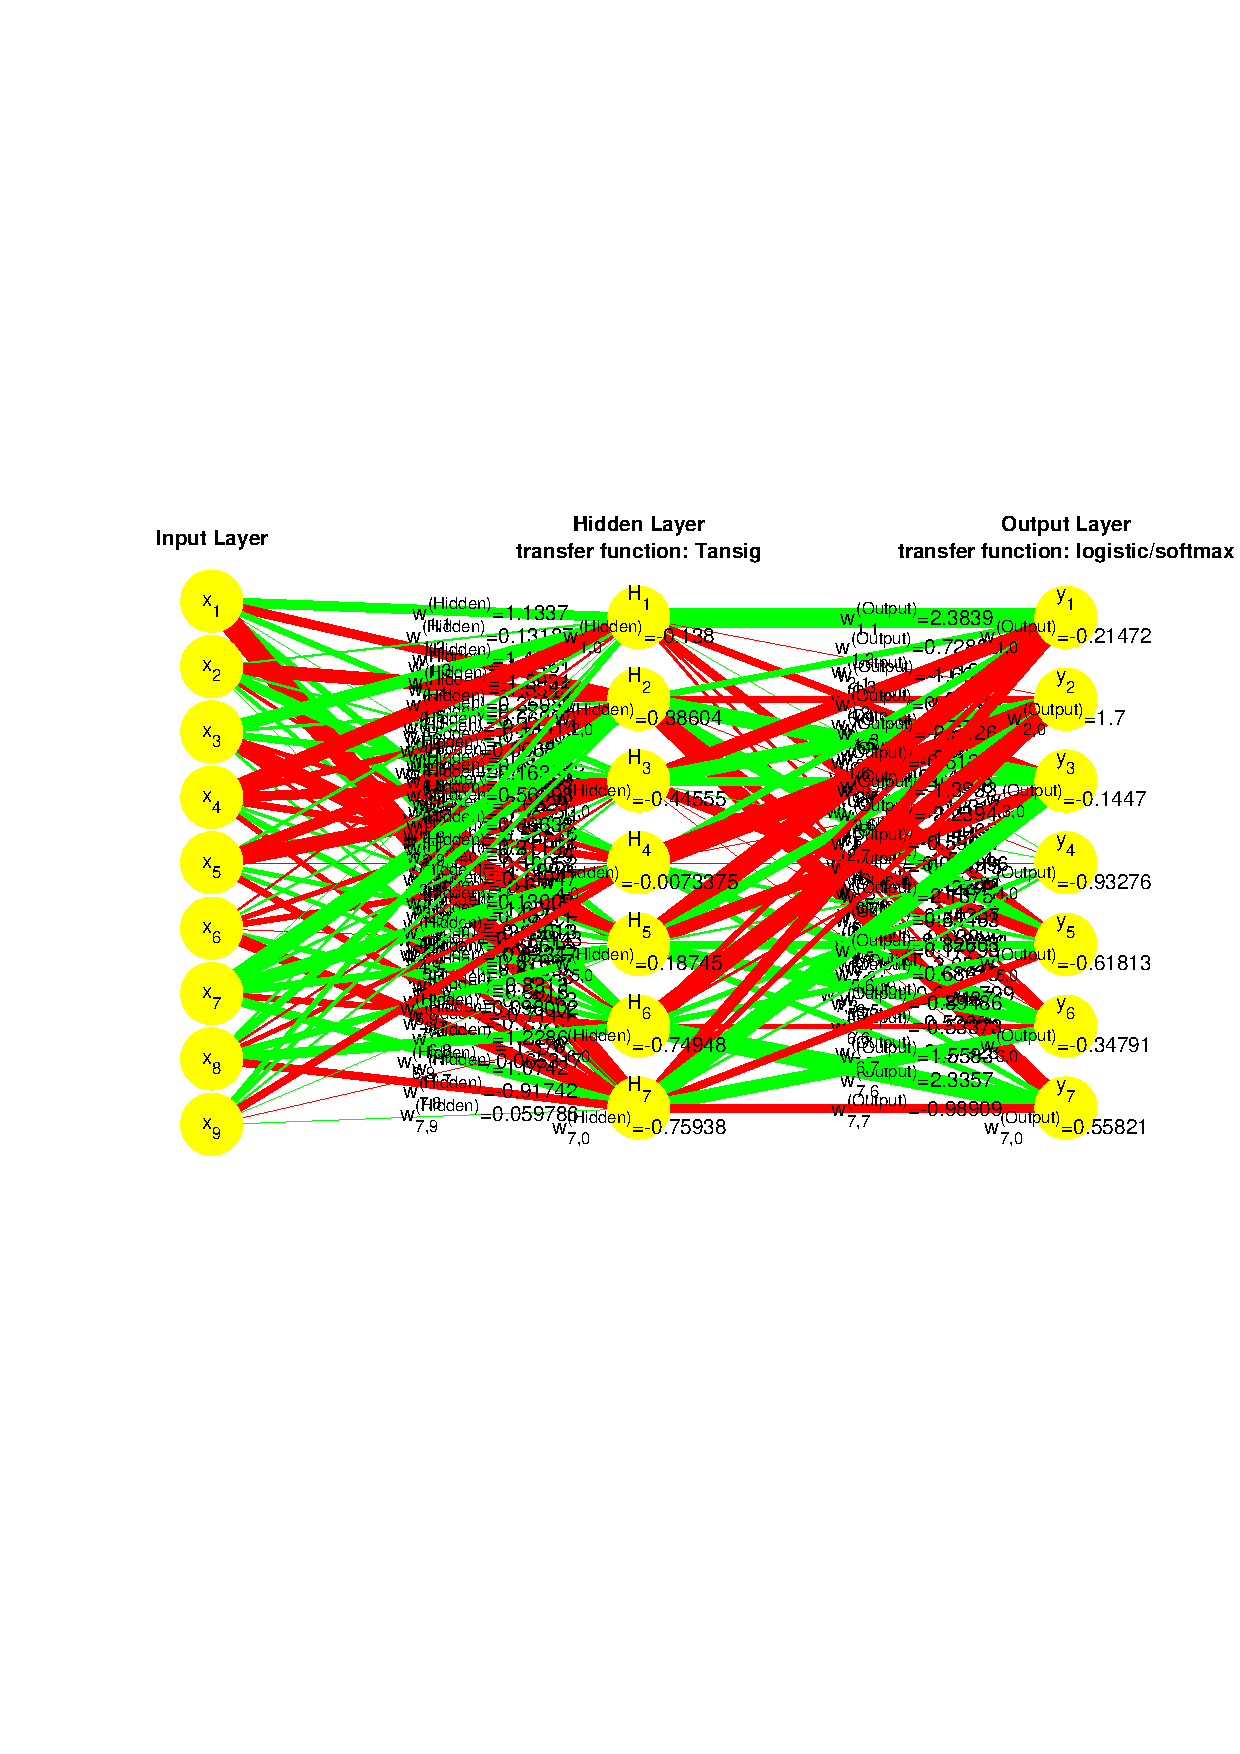
\includegraphics[width=1.0\textwidth]{fig/classification/ANN_class_trained_network.pdf}
    \caption{Visualization of the trained network in the ANN regression problem. We have 9 input variables (ratio weight percent attributes and RI), so there are $D=9$ input nodes. The inner CV loop selected $H=7$ as the optimal number of hidden nodes. The goal is to predict the probability of of the observation being type1 through type7, so there is $D = 7$ output nodes. The network contains so many nodes that the neural weights become unreadable. From the line widths between nodes, however, we notice that input variable 9 (refraction index \texttt{RI}) is the least important. This makes sense, as we found in the regression part of the report that \texttt{RI} can successfully be predicted from 8 chemical weight percent attributes (input nodes 1 through 8). }
\end{figure}